\documentclass[english,12pt,doc]{apa}
\usepackage[a4paper, left=25mm, right=40mm]{geometry}

\usepackage{apacite}
\usepackage{amsmath}

\usepackage{tikz}
\usepackage[german]{babel}
\usepackage{verbatim}
\usepackage{setspace}
\usepackage{graphicx}
\usepackage{caption}
\usepackage{prettyref}
\usepackage{titleref}

\onehalfspacing
\setlength{\parskip}{1em} % 1ex plus 0.5ex minus 0.2ex}
\setlength{\parindent}{0pt}

\usepackage[utf8]{inputenc}

\usepackage[]{blindtext}
\rightheader{Automatische Verfahren zur Prädiktorauswahl}

\begin{document}

\title{Automatische Verfahren zur Prädiktorauswahl in Regressionsmodellen}
\shorttitle{Prädiktorauswahl in Regressionsmodellen} 
\author{Literaturarbeit vorgelegt von \\ Markus Graf (markus.graf@uzh.ch)}
\date{\today}
\affiliation{am  Psychologisches Institut der Universität Zürich\\ Betreut durch Dr. Christina Werner}
\abstract{Eigener Abstract: - 

Themenvorgabe: In vielen psychologischen Bereichen geht es darum, Kriteriumsvariablen durch Prädiktorvariablen möglichst gut vorherzusagen. 
Wenn viele potentielle Prädiktorvariablen in Frage kommen und es keine theoretischen Gründe gibt, die nur ganz bestimmte Prädiktorvariablen nahelegen, werden in Anwendungssituationen oft automatische Verfahren der Auswahl von Prädiktorvariablen verwendet, um mit möglichst wenigen Prädiktoren eine möglichst gute Vorhersage des Kriteriums zu erreichen, beispielsweise die sog. ``Stepwise''-Methode in multiplen Regressionsmodellen. 
Die Literaturarbeit soll einen Überblick über verschiedene existierende Möglichkeiten zur Selektion von Prädiktorvariablen in Regressionsmodellen geben, und deren Eignung für psychologische Anwendungen kritisch diskutieren.}
\maketitle
\setlength{\parindent}{0pt}
\newpage
\tableofcontents
\newpage
\section{Einführung}
Das Standardverfahren um den quantitative Zusammenhang zwischen einer abhängigen und einer unabhängigen Variablen zu beschreiben stellt die Regressionsanalyse dar. 
Begründet wurde dieses Verfahren durch Carl Friedrich Gauss in seiner Schrift, in der er, mit Hilfe der Methode der kleinsten Quadrate, die Bewegung der Himmelskörper um die Sonne im Kegelschnitt beschrieb \cite{gauss1809theoria}. 

Im Unterschied zur einfachen linearen Regression, werden in einem multiplen Regressionsmodell mehrere unabhängige Variablen mit einbezogen. 
Es resultiert eine Regressionsgleichung welche zur Vorhersage einer Kriteriumsvariable aufgrund mehrerer Prädikatorvariablen genutzt wird  \cite[S. 448]{bortz2011}. 
Als Gretchenfrage stellt sich nun welche Prädikatoren nun ein Modell am besten erklären. 
Zu beginn der Psychologischen Forschung mussten Modelle von Hand berechnet werden. Zwangsläufig wurden wenige Prädikatoren erhoben und einfache Modelle Gerechnet. 
Friedman analysierte beispielsweise 1944 die Langlebigkeit von Turbinenschaufeln in Abhängigkeit von Stress, Temperatur und einigen Legierungsparametern. 
Zwar wurde die Berechnung nicht mehr von Hand durchgeführt, doch benötigte eine Regressionsschätzung inklusive Berechnung der Teststatistiken rund 40 Stunden \cite[p.2]{armstrong2011illusions}. Jeder durchschnittliche Computer erledigt dies heutzutage Sekundenbruchteile. 

Mit dem technische Fortschritt einhergehend wurden Verfahren entwickelt, welche möglichen Kombinationen von Prädiktoren berücksichtigen und gegeneinander testen. 
In einem ersten Teil dieser Arbeit werden die wichtigsten Verfahren dargestellt. 

Es können beliebig viele potentiell erklärende Variablen erhoben werden um sich komplexe Modell generieren zu lassen. 
Menschen tendieren zu glauben, dass komplexe Probleme komplexe Lösungen benötigen. 
Die Forschung zeigt jedoch, dass gerade das Umgekehrte der Fall ist \cite[p.3]{armstrong2011illusions}. 
Insbesondere Gigerenzer demonstrierte eindrucksvoll wie mit einfachen Rekognitionsheuristiken bessere Vorhersagen gemacht werden konnten als mit komplexen statistischen Modellen \cite{borges1999can}. 
Komplexe Modelle können sehr gute Vorhersagen liefern innerhalb des Trainingsdatensatz, doch oft scheiter die Vorhersage beim Versuch, diese zu generalisieren. 
Der zweite Teil befasst sich mit dem Problem der Überanpassung komplexer Modelle und diskutiert mögliche Lösungsansätze.

\section{Automatische Modellwahlverfahren}
In der psychologischen Forschung kommen oft Ex-post-facto-Designs zum Einsatz. 
Dies insbesondere weil viele Daten mit geringem Aufwand erhoben werden können. Oft werden  Daten gleich für mehrere Studien erhoben und in anderen Studien verwendet. 
Daraus resultieren viele potenzielle Prädikatorvariablen für neue Fragestellungen. 
Es gilt das ``beste'' Modell berechnen, oft ohne das es theoretische Gründe gibt nach denen die Auswahl der Prädiktoren einzuschränken ist.
``Alle Modelle sind falsch, aber einige sind nützlich'' \cite[p.202]{box1979robustness}.
Box will damit hervorheben, dass obschon in der Literatur oft vom ``besten'' oder ``wahren'' Modell gesprochen wird, dies nur ein Approximation darstellt \cite[p.172]{weakliem2004introduction}. 
\subsection{Exhaustiv Regression} 
Eine naive Herangehensweise ist alle möglichen Modelle welche mit $p$ Prädiktoren möglich sind durch zurechnen. 
Zur Beurteilung der Modellgüte kann die mittlere quadratische Abweichung herangezogen werden. 
Das ``beste'' Modell hat die kleinste mittlere quadratische Abweichung ($S_p$-Kriterium) \cite[p. 5]{thompson1978selection}. 
Da alle Möglichen Kombinationen durch gerechnet werden, wird das ``beste'' Modell, also das welches den Referenzdatensatz am besten Vorhersagen kann, gefunden. 
Entsprechend wird in der Literatur auch oft vom optimalen Modell gesprochen. Es liegt jedoch auf der Hand, dass dies zwar die interne Validität erhöht, aber die externe Validität gefährdet.
Das optimale Modell kann, insbesondere bei hoher Komplexität, zu fest auf die Referenzdaten behaftet sein und dadurch schlecht generalisierbar sein.
Auf diesen Effekt der Überanpassung wird im zweiten Teil dieser Arbeit noch näher eingegangen.  
\citeA[p.6]{thompson1978selection} sieht einzig den Nachteil darin, dass der Rechenaufwand exponentiell mit der Anzahl zu berücksichtigender Prädikatoren steigt. 
Es müssen immer $2^p-1$ Modelle berechnet werden, bei 5 Prädikatoren sind dies 31 Modelle, bei 10 bereits 1023 usw.
Während früher eingeschränkte Rechenkapazität oft ein ökonomischer Faktor war - es musste Rechenzeit in einem Rechenzentrum reserviert werden, spielt die Rechengeschwindigkeit auf modernen Systemen eine untergeordnete Rolle, da insbesondere in der Psychologie oft nur eine Handvoll Prädikatoren durch gerechnet werden müssen.

\subsection{Schrittweise Regression} Das optimale Modell beinhaltet jeden Prädikator, der die Voraussage bezüglich des getesteten Datensatzes auch nur minimal verbessert. 
Es stellt sich die Frage ob diese minimale Verbesserung noch nützlich ist. 
Die ``stepwise''-Verfahren arbeiten wesentlich liberaler, in dem Prädikatoren hinzugefügt oder eliminiert werden, je nach deren Relevanz für die Modellgüte. 
Es werden Kriterien festgelegt, nach welchen ein Modell als angemessen zu betrachten ist. 
Dies hat gegenüber der exhaustiven Verfahren den Vorteil, dass nicht alle Modelle berechnet werden müssen und entsprechend schneller Lösungen gefunden werden. 
Im Schnitt müssen xxxx Modelle berechnet werden, um eine adäquate Lösung zu finden \cite{tobecite}.

Innerhalb der schrittweisen Verfahren unterscheidet man zwischen \textit{forward selection} und \textit{backward elimination}. 
Ausgehend vom leeren Modell werden in der ersten Variante schrittweise weitere Variable der Nützlichkeit nach in das Modell integriert, bis eine Abbruchbedingung erfüllt ist. 
\begin{figure}[hb]
	\centering
	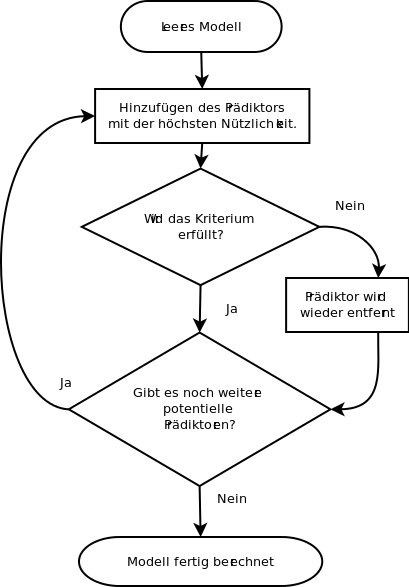
\includegraphics[width=\textwidth]{forward_stepwise.png}
	\caption{Forward Selection}
	\label{fig:forward_stepwise}
\end{figure}

In der zweiten Variante werden alle Prädikatoren in das Modell integriert und schlechte entfernt, wiederum bis das Kriterium erreicht ist. 
\begin{figure}[hbtb]
	\centering
	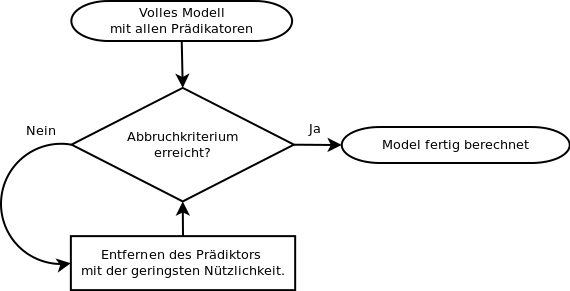
\includegraphics[width=\textwidth]{backward_stepwise.png}
	\caption{Backward Elimination}
	\label{fig:backward_stepwise}
\end{figure}

Die Aufnahme einer neuen Variable kann dazu führen, dass eine bereits im Modell vorhandene Variable obsolet wird. 
Um diesem Umstand Rechnung zu tragen werden oft forward selection und backward elimination kombiniert \cite[p. 461]{bortz2011}. 

In seltenen Fällen kann es vorkommen, dass zwei Variablen für sich das Kriterium in die Regressionsgleichung aufgenommen zu werden nicht erfüllen, jedoch zusammen zum Vorhersagepotential einen substantiellen Beitrag leisten \cite[p.261]{jacob2003applied}. 
Schrittweise Verfahren sind entsprechend nicht in der Lage solche Effekte mit zu berücksichtigen. 

Entgegen dem exhaustiven Verfahren besteht bei schrittweisen Verfahren das Problem, dass unter Umständen nicht das optimale Modell gefunden wird. 
Da die Nützlichkeitsunterschiede, welche oft nur geringe statistische Bedeutung haben, das Modell bestimmen, bezeichnet \citeA[p. 462]{bortz2011} dieses Verfahren eher zu den explorativen gehörend. 
\citeA[p. 56ff]{harrell2001regression} lehnt das Verfahren gar ab und führt ins Feld, dass sämtliche statistischen Prinzipien verletzt würden. 
\citeA{berk1978comparing} zeigte jedoch in einem Vergleich, dass die durchschnittliche Differenz der Fehlerquadratsummen zwischen exhaustiven und schrittweiser Regression kaum 7\% übertrifft. 

Zentrales Element der schrittweisen Regression ist das Mass zur Beurteilung der  Modellanpassung, welche besagt, weshalb und wann ein Modell als akzeptabel zu betrachten ist. 
Als Folge dessen wird damit auch die Anzahl relevanter Prädiktoren bestimmt.

\paragraph{Bestimmtheitsmass}  Das Quadrat des multiplen Korrelationskoeffizienten $R^2$ besagt wie viel systematische Varianz aufgeklärt wird. 
Je grösser die Zahl der unabhängigen Variablen ist, desto grösser wird das Bestimmtheitsmass, weshalb eine Korrektur vorgenommen werden muss. 
Insbesondere bei kleinem $R^2$ sollte auf Signifikanz getestet werden, entsprechend wird in schrittweisen Verfahren Prädikatoren nicht einzig aufgrund von $R^2$ selektiert. 

\paragraph{Signifikanztest} Das Verfahren wird beendet, wenn kein Prädikator mehr vorhanden ist, der das Vorhersagepotential signifikant erhöht \cite[p.48]{bendel1977comparison}. 
Das vergleichen zweier Regressionsgleichungen mittels Signifikanztest bedingt, dass diese geschachtelt sein müssen, das kleinere Modell muss im grösseren enthalten sein \cite[p. 508]{jacob2003applied}.

Das gewählte Signifikanzniveau ist eigentlich unbegründet gewählt \cite[p. 174]{weakliem2004introduction}. \citeA[p. 269]{derksen2011backward} diskutieren mehrere Empfehlungen für Signifikanzniveaus und weisen darauf hin, das sich über mehrere Tests der $\alpha$-Fehler kumuliert. 
In  Simulationen mit artifiziellen Daten zeigen \citeA{mundry2009stepwise} das  Problem multipler Tests beispielhaft auf. 
Daraus resultierend lehnen sie die Verwendung der schrittweisen Regression gar ab.

Ein weitere Schwäche des Hypothesentestens ist der Einfluss der Stichtprobengrösse. So kann bei genügend grossem Umfang nahezu jede Hypothese abgelehnt werden, was wiederum zu komplexen und überangepassten Modellen führt \cite[p.173]{weakliem2004introduction}.

\subsection{Multikollinearität}
Multikollinearität, als hohe Korrelationen zwischen mehreren Prädikatoren, führt zu Problemen bei der automatischen Modellwahl. 
In schrittweisen Verfahren ist es in solchen Fällen häufig vom Zufall abhängig welche der beteiligten Variablen als erste weggelassen beziehungsweise aufgenommen wird. 
Ein Anstieg der  korrelation zwischen Prädiktoren hat zur Folge, dass (a) die p-Werte bei Signifikanztests sinken, (b) schwache Prädiktoren entgegen den starken eher fälschlicherweise ausgeschlossen werden, (c) korrekt hoch signifikante Prädiktoren werden eher ausgeschlossen wenn die korrelation zwischen einem konfundierenden Prädiktor und dem Kriterium steig und (d) selbst wenn die korrelation zwischen konfundierendem Prädiktor und Kriterium klein ist, besteht die Gefahr, dass korrekt schwach signifikante Prädiktoren nicht signifikant werden \cite[p. 2810]{graham2003confronting}.

Grundsätzlich gilt die Unabhängigkeit der Prädikatoren als Voraussetzung für die multiple Regression, doch gerade in der psychologischen Forschung lassen sich Korrelationen meist schlecht vermeiden.
Um bereits im Vorfeld Hinweise auf potentielle Kollinearität zu erhalten, empfiehlt es sich die Kovarianzmatrix zwischen allen Prädikatoren vor der eigentlichen Auswahl zu betrachten.
Eventuell wurde das selbe Merkmal mehrmal erhoben.
Der Zusammen hang zwischen den Prädikatorvariablen und der vorhergesagten Kriteriumsvariable lässt sich mit dem Strukturkoeffizienten $c_i$ ausdrücken. So kann auf die Prädikatoren eingeschränkt werden,  welche am besten das Kriterium vorhersagen \cite[S. 453]{bortz2011}. 

\section{Überanpassung - Der einfachste Ausdruck verwickelter Probleme ist immer der beste}
\label{sparsamkeit}
Der Mensch strebt nach Kontrolle und verfällt dabei oft der Illusion, alles bis ins letzte Detail kontrollieren zu müssen.
Entsprechend wurden im Zuge der technischen Revolution hoch komplexe Systeme und Maschinen entwickelt, welche jeder Anwendung gerecht werden sollten. 
Insbesondere im Bereich des Produktdesigns hat in den letzten Jahren ein radikales umdenken statt gefunden: ``Simplicity is about subtracting the obvious, and adding the meaningful.'' \cite{maeda2006laws}. Einfachheit wurde gelebt was zahlreiche unumstritten grossartige Produkte hervor brachte. 

Die Illusion der Komplexität ist auch in der Statistik anzutreffen \cite[p. 3]{armstrong2011illusions}. 
Im Kontext der Modellwahl äussert sich dies in Form der Überanpassung, wenn also das Modell zu sehr an die Testdaten angepasst ist.
Insbesondere Modelwahlverfahren, welche die Anzahl der Prädikatoren nicht abstrafen, sind davon betroffen.
Als Einflussfaktoren seitens der Daten sind Representativität und Stichprobengrösse zu nennen. 
Mit steigendem Stichprobenumfang und höheren Repräsentativität sinkt die Überanpassung und steigt die stabilität der Vorhersage.


\subsection{Kriterienbasierte Strategien}
Die bisher beschriebenen Modellwahlverfahren fokusieren sich darauf anhand der gegebenen Daten das ``beste'' Modell zu finden.
Kriterienbasierende Strategien zur Vermeidung der Überanpassung strafen komplexität ab, in dem das Kriterium diese berücksichtigt.
Je komplexer ein Regressionsmodell wird, desto besser muss die Vorhersage stimmen um die komplexität zu rechtfertigen.

Colin Lingwood Mallows entwickelte das $C_p$ Kriterium, dass auf der Methode der kleinsten Quadrate ($S_p$-Kriterium) aufbaut und sowohl die Prädikatoranzahl als auch die Stichprobengrösse berücksichtigt. Angestrebt wurde dabei alle wichtigen Prädikatoren zu berücksichtigen. 
Das ``beste'' Modell ist das mit (a) dem niedrigsten Cp-Wert, der (b) möglichst gleich p ist, ist \cite{gilmour1996interpretation}.

EINFüHREND \cite[p.170]{weakliem2004introduction}

Das Akaikes Informationskriterium (AIC) und Bayessche Informationskriterium (BIC) basieren auf der Maximum-Likelihood-Methode, Regressionsgleichungen müssen nicht ineinander geschachtelt sein und der Kennwert berücksichtigen die Komplexität des Modells anhand der Prädiktoranzahl. 
Die beiden Kennwerte strafen dem Prinzip der Sparsamkeit entsprechend Komplexität, was der Überanpassung entgegen wirkt.

Das schrittweise Verfahren stoppt, wenn die Grösse AIC / BIC nicht mehr abnimmt.


\subsection{Kreuzvalidierung}
Die Stabiltität eines Modelles lässt sich durch den Vergleiche mit zusätzlichen Stichproben ermitteln.
Zu diesem Zweck kommen sogenannte Kreuzvalidierungsverfahren zum Einsatz.

Die Idee hinter der Kreuzvalidierung liegt darin, die Daten aufzuteilen. Zum einen in eine Referenzstichprobe, anhand der die Gleichung geschätzt wird, zum anderen in eine oder mehrere zusätzliche Teststichproben, anhand dererer die Stabilität als durchschnittliche Fehlerquote berechnet wird \cite[p. 3]{arlot2010survey}.

Es frag sich welchen Platz die Kreuzvalidierung in der Modellselektion einnimmt.
Kreuzvalidierungen können über ein Set von $n$ Regressionsgleichungen durchgeführt werden, beispielsweise  potentielle Modelle nach einer schrittweisen Regression \cite[p. 12]{arlot2010survey}.
$n$ potentiellen Modelle werden validiert, wobei unter Umständen das stabilste nicht gleich dem vielversprechendsten aus der vorangegangenen Selektion ist.
 Überangepasste Modelle können somit eliminiert werden und an deren Platz rücken einfachere und stabilere Modelle.
Der Vorteil dieses Vorgehens liegt darin das (a) die Validierung komplett von der Modellselektion getrennt werden kann und (b) es nur $n$ Durchgänge benötigt. 
In der Modellselektion wird jedoch die stabilität nicht berücksichtigt. 
Bei der schrittweisen Regression haben wir gesehen, dass das ``beste'' Modell nicht zwangsläufig gefunden wird.
Entsprechendes gilt für die Stabilität, was zur Konsequenz führen kann, dass zwar gute Modelle gefunden werden, diese jedoch allesamt nicht stabil genug sind oder das stabilste schlicht nicht gefunden wird. 
\citeA[p. 12]{arlot2010survey} nennen noch die Möglichkeit die Stabilität in die Modellselektion zu integrieren und als  Kriterium zu berücksichtigen. 
Zu jeder Modellschätzung wird deren Stabilität berechnet und Modelle welche keine genügenden Werte aufweisen werden abgewiesen. Ein Nachteil dessen ist der höhrere Rechenaufwand, da für jedes Modell zusätzliche Durchgänge benötigt.

Kreuzvalidierungsverfahren unterscheiden sich in erster Linie anhand der Strategie, mit der die Daten ``getrennt'' werden.
In der Regel wird dafür ein genug grosser Datensatz herangezogen und unterteilt, wobei vorausgesetzt wird, dass die Teilstichproben unabhängig und gleich verteilt sind. 
Bei $k$-Facher-Kreuzvalidierung wird der Datensatz in $k$ möglichst gleich grosse Teile aufgeteilt und $k$ Testläufe durchgeführt.
 Der Durchschnitt aus den Einzelfehlerquoten der k Durchläufe entspricht der Gesammtfehlerquote welche für jede Lösung verglichen werden kann \cite[p. 14]{arlot2010survey}.
Je niedriger die Gesammtfehlerquote, desto stabiler ist die Regressionsgleichung.
Um der gleichverteilung der Untermengen gerecht zu werden diese gelegentlich auch stratifiziert \cite{diamantidis2000unsupervised}. 
Weitere Verfahren und deren Vergleiche finden sich bei \citeA{arlot2010survey}.

Die Kreuzvalidierung ist ein gutes Mittel um Überanpassung entgegen zu wirken.
Darüber hinaus ist die Stabilität ein guter Indikator für die Generalisierbarkeit.
Bedingung ist jedoch, dass dadurch zusätzlich Datensätze zur Verfügung stehen, was im bereich der Psychologischen Forschung durchaus nicht immer gegeben ist.

\section{Software zu den vorgestellten Verfahren}
Die bisher vorgestellten Verfahren sind in den meisten grösseren Statistikprogrammen bereits integriert oder können als Erweiterung hinzugefügt werden.
Insbesondere wenn es darum geht verschiedene Verfahren der Modellseleketion zu beurteilen bietet sich R an.

R ist eine frei verfügbare Programmiersprache für statistisches Rechnen und setzt momentan den Standart im Bereich der Rechnergestützten Datenanalyse. 
Eine guter Einstieg in R, mit vielen interaktiven Übungen, bietet der Kurs ``tryR''\footnote{http://tryr.codeschool.com} von code school.
Für das tägliche Arbeiten mit R ist  \citeA{R:Teetor:2011a} empfehlenswert.

\subsection{Modellselektion}
Das exhaustive Verfahren wurde im Paket ``leaps'' von \citeA{R:leaps} implementiert. 
Ausgegeben werden kann Mallows's $C_p$, $R^2$ oder auch das adjustierte Bestimmtheitsmass $\bar R^2$.

Die schrittweise Regression ist ein fester Bestandteil von R \cite{R:core} und ermöglich eine bestehende Gleichung schrittweise vorwärts, rückwärts oder beidseitig zu durchsuchen.
Als Kriterium wird dabei Akaikes Informationskriterium verwendet, da $step(object, ...)$ eine vereinfachte Implementierung der Funktion $stepAIC(object, ...)$  aus dem Paket ``MASS'' darstellt \cite{R:MASS}. 
Aussführlicher werden die kriteriumsbasierende Verfahrens mit R bei \citeA{faraway2002practical} beschrieben.

\subsection{Kreuzvalidierung}
Für die $k$-Fache-Kreuzvalidierung bietet sich die Funktion $CVlm(...)$ aus dem Paket ``DAAG'' an \cite{R:DAAG}. 
Die Funktion bietet über die reine Berechnung hinaus die Möglichkeit die $k$ Durchgänge grafisch auszugeben.


\section{Zusammenfassung / Diskussion} 


\blindtext

\newpage
\bibliographystyle{apacite} 
\bibliography{literature}
\newpage
\section{Anhang}
\blindtext
\newpage
\section{Selbstständigkeitserklärung}
\blindtext
\begin{comment}

\\
\\
Name: Markus Graf\\
Matriculation number:  08-91271-9\\
\\
\\
\\
\\
\\
\\
............................................................................\\
Zürich, \today
\end{comment}


\end{document}
